\begin{figure}[!tbp]
\centering
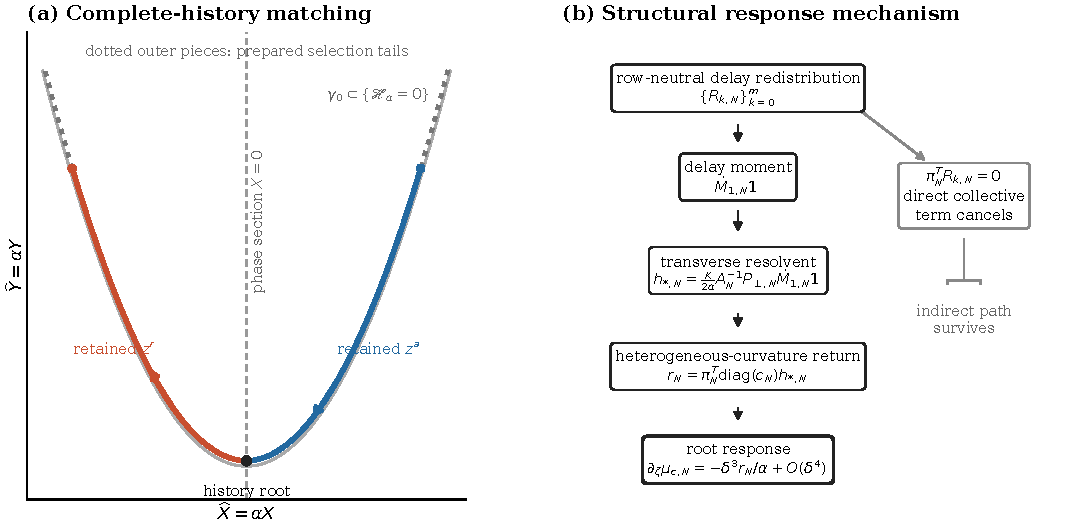
\includegraphics[width=.94\textwidth]{figures/root-mechanism.pdf}
\caption{\textbf{Projection-blind return and the anchored heteroclinic-canard
root.}
\textup{(a)} Schematic history-space projection for one fixed anchored RFDE:
the incoming branch tracks attracting and repelling slow-history graphs and
then enters the intrinsic stable sheet of \(E_N^-\).  The shaded tube is where
the anchored and original equations agree exactly; positions are not
quantitative.  \textup{(b)} Proved information path.  Two separated delays
make the blind source onto, whereas one merged delay gives the leading
first-moment no-go; the returned covector is the root derivative.
\textup{(c)} Schematic root graphs for two anchors.  Absolute roots may differ,
but modelwise centering and \(\delta^{-3}\) scaling give the common tangent
\(\Lambda_N(R)+O(\delta)\) and limiting conormal
\(\mathrm d\xi-\Lambda_N(R)\mathrm d\zeta\).  No root for the unanchored law,
or equality across anchors, is asserted.}
\label{fig:root-mechanism}
\end{figure}
